%%%%%%%%%%%%%%%%%%%%%%%%%%%%%%%%%%%%%%%%%%%%%%%
%
% Template per Elaborato di Laurea
% DISI - Dipartimento di Ingegneria e Scienza dell’Informazione
%
% update 2015-09-10
%
% Per la generazione corretta del
% pdflatex nome_file.tex
% bibtex nome_file.aux
% pdflatex nome_file.tex
% pdflatex nome_file.tex
%
%%%%%%%%%%%%%%%%%%%%%%%%%%%%%%%%%%%%%%%%%%%%%%%

% formato FRONTE RETRO
\documentclass[epsfig,a4paper,11pt,titlepage,twoside,openany]{book}
\usepackage{epsfig}
\usepackage{plain}
\usepackage{siunitx}
%\usepackage[T1]{fontenc}
\usepackage{setspace}
\usepackage[paperheight=29.7cm,paperwidth=21cm,outer=1.5cm,inner=2.5cm,top=2cm,bottom=2cm]{geometry} % per definizione layout
\usepackage{titlesec} % per formato custom dei titoli dei capitoli
\usepackage{cleveref}
\usepackage{tabu}
\usepackage{amsmath}
\usepackage{float}
\usepackage{relsize}
\usepackage[ruled]{algorithm2e}
\usepackage{fixltx2e}
\usepackage{listings}
%%%%%%%%%%%%%%
% supporto lettere accentate
%
%\usepackage[latin1]{inputenc} % per Windows;
\usepackage[utf8x]{inputenc} % per Linux (richiede il pacchetto unicode);
%\usepackage[applemac]{inputenc} % per Mac.

\singlespacing

\usepackage[american]{babel}

\begin{document}

  % nessuna numerazione
  \pagenumbering{gobble}
  \pagestyle{plain}

\thispagestyle{empty}

\begin{center}
  \begin{figure}[h!]
    \centerline{
\psfig{file=fig/logo_unitn_black_center.eps,width=0.6\textwidth}}
  \end{figure}

  \vspace{2 cm}

  \LARGE{Dipartimento di Ingegneria e Scienza dell’Informazione\\}

  \vspace{1 cm}
  \Large{Corso di Laurea in\\

    Informatica
    %Ingegneria dell'Informazione e delle Comunicazioni
    %Ingegneria dell'Informazione e Organizzazione d'Impresa
    %Ingegneria Elettronica e delle Telecomunicazioni
  }

  \vspace{2 cm}
  \Large\textsc{Elaborato finale\\}
  \vspace{1 cm}
  \Huge\textsc{Markovian models for Vehicular Networks\\}


  \vspace{2 cm}
  \begin{tabular*}{\textwidth}{ c @{\extracolsep{\fill}} c }
  \Large{Supervisor} & \Large{Graduand}\\
  \Large{Prof. Renato Antonio Lo Cigno}& \Large{Pierfrancesco Ardino}\\\\
  \Large{Co-Supervisor} & \\
    \Large{Michele Segata}& \\
  \end{tabular*}

  \vspace{2 cm}

  \Large{Anno accademico 2014/2015}

\end{center}



  \cleardoublepage

%%%%%%%%%%%%%%%%%%%%%%%%%%%%%%%%%%%%%%%%%%%%%%%%%%%%%%%%%%%%%%%%%%%%%%%%%%
%%%%%%%%%%%%%%%%%%%%%%%%%%%%%%%%%%%%%%%%%%%%%%%%%%%%%%%%%%%%%%%%%%%%%%%%%%
%% Nota
%%%%%%%%%%%%%%%%%%%%%%%%%%%%%%%%%%%%%%%%%%%%%%%%%%%%%%%%%%%%%%%%%%%%%%%%%%
%% Sezione Ringraziamenti opzionale
%%%%%%%%%%%%%%%%%%%%%%%%%%%%%%%%%%%%%%%%%%%%%%%%%%%%%%%%%%%%%%%%%%%%%%%%%%
%%%%%%%%%%%%%%%%%%%%%%%%%%%%%%%%%%%%%%%%%%%%%%%%%%%%%%%%%%%%%%%%%%%%%%%%%%
  \thispagestyle{empty}

\begin{center}
  {\bf \Huge Ringraziamenti}
\end{center}

\vspace{4cm}


\emph{
  ...thanks to...
}

  \cleardoublepage
  \pagestyle{plain} % nessuna intestazione e pie pagina con numero al centro


  % inizio numerazione pagine in numeri arabi
  \mainmatter

%%%%%%%%%%%%%%%%%%%%%%%%%%%%%%%%%%%%%%%%%%%%%%%%%%%%%%%%%%%%%%%%%%%%%%%%%%
%%%%%%%%%%%%%%%%%%%%%%%%%%%%%%%%%%%%%%%%%%%%%%%%%%%%%%%%%%%%%%%%%%%%%%%%%%
%% Nota
%%%%%%%%%%%%%%%%%%%%%%%%%%%%%%%%%%%%%%%%%%%%%%%%%%%%%%%%%%%%%%%%%%%%%%%%%%
%% Si ricorda che il numero massimo di facciate e' 30.
%% Nel conteggio delle facciate sono incluse
%%   indice
%%   sommario
%%   capitoli
%% Dal conteggio delle facciate sono escluse
%%   frontespizio
%%   ringraziamenti
%%   allegati
%%%%%%%%%%%%%%%%%%%%%%%%%%%%%%%%%%%%%%%%%%%%%%%%%%%%%%%%%%%%%%%%%%%%%%%%%%
%%%%%%%%%%%%%%%%%%%%%%%%%%%%%%%%%%%%%%%%%%%%%%%%%%%%%%%%%%%%%%%%%%%%%%%%%%

    % indice
    \tableofcontents
    \cleardoublepage



    % gruppo per definizone di successione capitoli senza interruzione di pagina
    \begingroup
      % nessuna interruzione di pagina tra capitoli
      % ridefinizione dei comandi di clear page
     % \renewcommand{\cleardoublepage}{}
     % \renewcommand{\clearpage}{}
      % redefinizione del formato del titolo del capitolo
      % da formato
      %   Capitolo X
      %   Titolo capitolo
      % a formato
      %   X   Titolo capitolo

      \titleformat{\chapter}
        {\normalfont\Huge\bfseries}{\thechapter}{1em}{}

      \titlespacing*{\chapter}{0pt}{0.59in}{0.02in}
      \titlespacing*{\section}{0pt}{0.20in}{0.02in}
      \titlespacing*{\subsection}{0pt}{0.10in}{0.02in}

      % sommario
      \chapter*{Extended abstract} % senza numerazione
\label{sommario}
\addcontentsline{toc}{chapter}{Extended abstract} % da aggiungere comunque all'indice


Mobile Ad-hoc NETworks are defined as a system of mobile nodes connected with each other via a wireless connection.
In this topic, Vehicular Ad-hoc NETworks are a particular case of MANETs where the nodes are vehicles equipped with communication devices. The idea of exchange information between static nodes and vehicular nodes has brought standardization bodies and automotive manufacturers to pay attention to its deployment and development.\vskip 1em
Applications in Vehicular communication networks can be classified into different categories. The two main categories are Vehicular-to-Vehicular communications (V2V) and Vehicular-to-Infrastructure  communications (V2I). In the first category the vehicles can set up an Independent Basic Service Set  without a controlling access point, exchanging information about traffic, speed, position and so on and so forth. Also, the vehicle can send information about problems in the car or problems with the driver to surrounding vehicles.\vskip 1em
In the second category, an Road side unit (RSU) can act as an access point with the Internet and forming a Basic Service Set with the vehicles in the network. Public authorities can use the data exchanged by the RSU with the vehicles in order to ease traffic flow and provide a real time response to congestion.\vskip 1em
IEEE 802.11p \cite{jiang2008ieee} is one of the recent amendments to the IEEE 802.11 standard that enables wireless access in vehicular environments (WAVE). IEEE 802.11p provides the basic radio standard for Dedicated Short Range Communications (DSRC). It is limited by the scope of IEEE 802.11, which is a MAC and PHY layer standard meant for single physical channel operation.The DSRC multi-channel setup and the operational concepts are taken care of by the upper layer IEEE 1609.
\vskip 1em
Another topic which gathers much interest is the performance measurement of realistic simulations of IVC protocols. An ideal scenario is to perform outdoor experiments, but setting the network and running an outdoor scenario can be dangerous and expensive. \vskip 1em
To overcome these problems, network simulation environments are commonly used to simulate the protocols before they are deployed in the real world. The quality of the results obtained by simulations is heavily influenced by the quality of the mobility models. There are different steps in the evolution of mobility models. At the beginning they relied on relatively simple models using random node movement. Later a crucial step was made using pre-recorded real-world mobility trace. These traces were obtained in outdoor experiments. While such a mobility model will arguably result in the most realistic vehicle movement in network simulations, its use is limited by this approaches’ inherent limitation to a small set of mobility parameters. Changing only one parameter, e.g. the density of vehicles, and keeping all other parameters unchanged is simply
infeasible in reasonably large scenarios. These problem can be overcome by generating these traces artificially. \\
In case where information about road conditions or warnings are transmitted over the network, a strictly interaction between the road traffic simulation and the network traffic is needed. In bidirectional simulations, two inter-dependent processes are running concurrently, the network simulator and the road traffic simulator. The two processes share information like position and speed of the simulated nodes, while other data are local.\newpage
A reason that made it really interesting to examine Vehicular Network is that they seem a credible opportunity to resolve traffic congestions, accidents, gives authorities real time information and so on and so forth. \\
This thesis aims to develop a Markov model based on the Gilbert model \cite{gilbert1960capacity}, a two state hidden Markov chain, in order to decrease the computational time used by the Veins framework \cite{sommer2011bid} to decode an incoming packet without losing accuracy. To do so, the new model is implemented and compared in term of time and accuracy with the actual model. \vskip 1em
\Cref{cha:VN} provides and introduction to the field of Vehicular Networks, their applications and the communication technologies used in this field.\\
\Cref{cha:frame} provides an introduction to the mobility models and their evolutions, the importance of network simulations to test new protocol before they are deployed in the real world. Furthermore, \Cref{cha:frame} introduces the frameworks used in this thesis. These are:
\begin{itemize}
    \item Veins: an open source Inter-Vehicular Communication simulation framework composed of an    event-based network simulator and a road traffic micro simulation model. The framework use OMNeT++ as network simulator and SUMO as road traffic simulator. Veins provides a comprehensive suite of IVC-specific models that can serve as a modular framework for simulating applications.
    \item SUMO: a microscopic road traffic simulators that uses the SK mobility model. SUMO allows high.performance simulations of huge networks with road consisting of multiple lanes, as well as intrajunction traffic on these roads. Vehicle types are freely configurable with each vehicle following statically assigned routes, dynamically generated routes, or driving according to a configured timetable.
    \item OMNeT++: a discrete event simulator for modeling communication networks, multi-processors and other distributed or parallel systems. Simulations are either run interactively, in a graphical environment, or are executed as command-line applications. The INET Framework extension used in Veins, provides provides a set of OMNeT++ modules that represent various layers of the Internet protocol suite, e.g., the TCP, UDP, IPv4, and ARP protocols.
\end{itemize}
\Cref{cha:PS} firstly provides an introduction to the mathematics background of the thesis, introducing the channel communications and the characteristics of a wireless signal. Then, it introduces the definition of Markov chain, the original model developed by Gilbert and a first possible solution to transform the model in a range-dependent Gilbert model. This because having the same parameters for each distance do not represent the characteristics of a communication link, which is strongly dependent on the distance. Then the network stack of the Veins framework is explained. As it explained in \Cref{sec:prob} the computation of the SNR and the SINR can be really expensive in large scenario with an high number of cars. The model proposed in this thesis aims to reduce the computation time by introducing an range-and-neighbors dependent Gilbert model. The changes made to the Veins framework are explained in \Cref{sec:implementation}.
\Cref{cha:eva} provides the evaluation of the new model. The scenario used is based on PLEXE \cite{segata2014plexe}, an extension of Veins which permits the realistic simulation of platooning protocols. Firstly, to estimate the parameters of the new model, three scenarios have been simulated, the first with 160 vehicles in the network, the second with 320 vehicles and the last with 640 vehicles. Each simulation has been repeated 10 times with different seeds for the generation of the random numbers. At the end only the simulations with 640 nodes has been used for estimating the parameter since it is the one that gives the best results.\\
As can be seen in \Cref{sec:estimation} a script has been used to extrapolate the data from the simulations and estimate the parameters of the new model.\\
The two models have been compared using two metrics, the efficiency and the accuracy of the results.
For the first metric the computation time of the two models have been computed.
As can be seen in \Cref{sec:gain}, the new model substantially decrease the computational time of the original model. \Cref{tab:duration} shows that there is a gain of the $76\%$ in execution time using the new model instead of the first, but this gain is useless if there is a low accuracy between the two models.
The second analysis analyze the accuracy between the two models. To measure the accuracy, the Packet Delivery Rate of the two models is computed and then the differences of packets exchanged by the two models has been measured using the sample mean and the standard deviation.
As can be seen in \Cref{sec:Resultaccuracy}, the result of the sample mean indicates that the original model correctly decoded in average $0.19\%$ packets more than the new model, while the result of the standard deviation indicates that there is only a deviation of $11.62\%$ from the sample mean.
In conclusion, it can be said that the new model is much faster than the original model without losing accuracy. The two models can be used together, the original model can be used in short simulations to estimate the parameters and then the new model can be used in long simulations saving up to days in computation times.\\
The contribution of the graduand for the work done in this thesis is determined by the implementation of the new model and the evaluation of it.
\newpage

      \cleardoublepage
%%%%%%%%%%%%%%%%%%%%%%%%%%%%%%%%%%%%%%%%%%%%%%%%%%%%%%%%%%%%%%%%%%%%%%%%%%
%%%%%%%%%%%%%%%%%%%%%%%%%%%%%%%%%%%%%%%%%%%%%%%%%%%%%%%%%%%%%%%%%%%%%%%%%%
%% Nota
%%%%%%%%%%%%%%%%%%%%%%%%%%%%%%%%%%%%%%%%%%%%%%%%%%%%%%%%%%%%%%%%%%%%%%%%%%
%% Sommario e' un breve riassunto del lavoro svolto dove si descrive
%% l’obiettivo, l’oggetto della tesi, le metodologie e
%% le tecniche usate, i dati elaborati e la spiegazione delle conclusioni
%% alle quali siete arrivati.
%% Il sommario dell’elaborato consiste al massimo di 3 pagine e deve contenere le seguenti informazioni:
%%   contesto e motivazioni
%%   breve riassunto del problema affrontato
%%   tecniche utilizzate e/o sviluppate
%%   risultati raggiunti, sottolineando il contributo personale del laureando/a
%%%%%%%%%%%%%%%%%%%%%%%%%%%%%%%%%%%%%%%%%%%%%%%%%%%%%%%%%%%%%%%%%%%%%%%%%%
%%%%%%%%%%%%%%%%%%%%%%%%%%%%%%%%%%%%%%%%%%%%%%%%%%%%%%%%%%%%%%%%%%%%%%%%%%

      %%%%%%%%%%%%%%%%%%%%%%%%%%%%%%%%
      % lista dei capitoli
      %
      % \input oppure \include
      %
      \chapter{Vehicular networks}
\label{cha:VN}
\section{Introduction to vehicular networks}
A Mobile Ad-hoc NETwork (MANET) \cite{abolhasan2004review} is defined as a system of mobile nodes, each connected by a wireless connection which can form a graph of an arbitrary structure. These nodes can move independently in every direction or follow a path.
Ad-hoc networks can be built on the spot and used in different kind of scenarios because they do not need a specific infrastructure. The growth of wireless communications led this topic to be one of the most important field of research from the middle of the 1990s.\vskip 1em
A particular case of MANETs are the \textit {Vehicular Ad hoc NETworks} (VANETs), which are a form of wireless ad hoc networks where nodes are vehicles equipped with communication devices that allow them to exchange messages with each other.
In VANETs there are two types of communication: Vehicle-to-Vehicle communication (V2V) and Vehicle-to-Infrastructure communication (V2I) where vehicles exchange messages with roadside network infrastructures (RSU). For example, \Cref{fig:vanet} \cite{Sanguesa2015vanet} shows the possible connections that can occur between nodes in a VANET.
\begin{figure}[H]
    \centering
    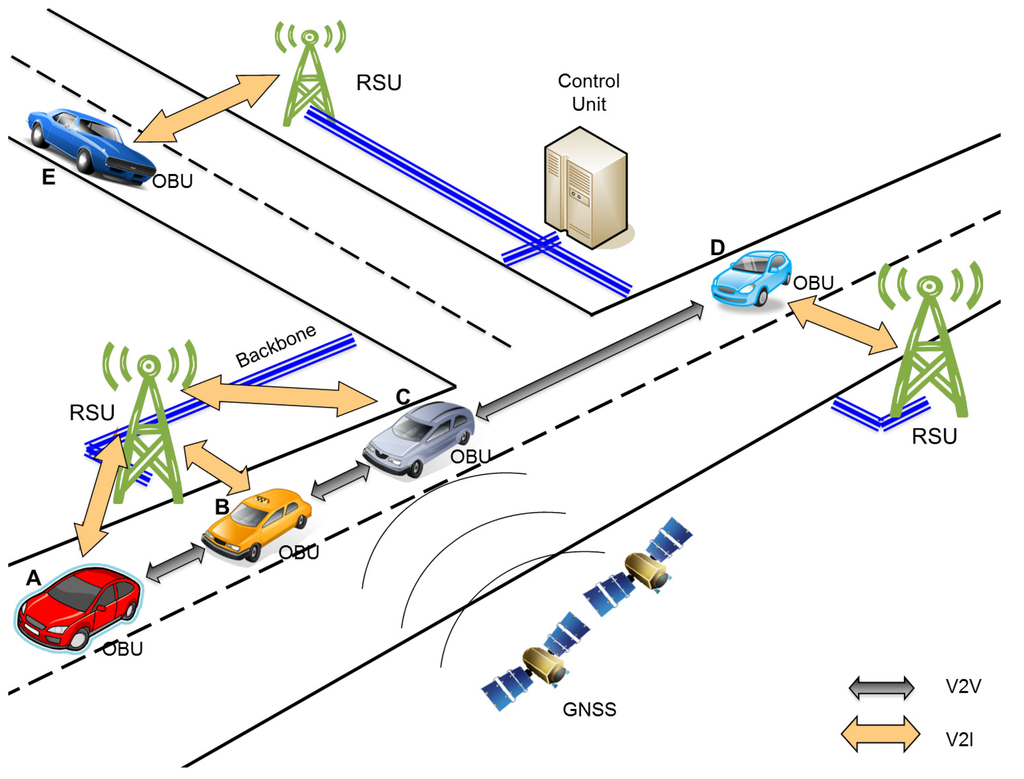
\includegraphics[width=0.6\textwidth]{fig/vanet.png}
    \caption{A representation of V2I and V2V connections}
    \label{fig:vanet}
\end{figure}
In the early 2000s VANETs were seen as an application of MANET principles but they soon became a research field on its own. Being the basis for what we call Inter-Vehicle-Communication \cite{ivc} (IVC), today the term is still somewhat synonymous with IVC, but it focuses on spontaneously created ad hoc networks and less on using pre-deployed infrastructure like RSUs.\vskip 1em
Several major automobile manufacturers have already begun to invest in real inter-vehicle networks and  have joined to create a non-profit organization called \textit {Car2Car Communication Consortium} (C2CCC) \cite{c2ccc} in order to increasing road traffic safety and efficiency by means of IVC.
\section{Application}
\label{sec:appl}
Here the concepts of operation for applications used in VANET systems are presented.
Applications can be classified into two main categories: vehicle-to-vehicle and infrastructure-to-vehicle applications.
Although most implementations of V2V applications only warn the driver of imminent collision or danger, the use of autonomous vehicle actions like braking or steering can be an important field of research in future systems.
\subsection{V2I applications}\vskip 1em
\label{subsec:V2I}
\textbf {Intersection violation warning} \vskip 1em
The intersection violation warning (IVW) application warns drivers when the violation of a red light seems imminent. A roadside unit co-located with a traffic light controller will broadcast information about location, light phase, light timing and intersection geometry to vehicles which are going to approach the intersection.
Vehicles then can compare this information with their trajectories and determine whether a signal violation is imminent. If so, the driver will be alerted and a signal is sent to the traffic light and surrounding vehicles to inform that a warning has been issued. \Cref{fig:ivwsafety}  \cite{hartenstein2010vanet} shows the violation of a red light.
\begin{figure}[H]
    \centering
    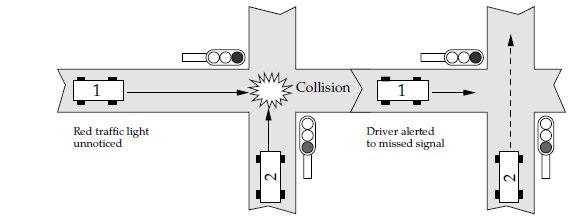
\includegraphics[width=0.75\textwidth]{fig/Ivw.png}
    \caption{Without IVW the driver will not be notified and so an accident can occur, while with IVW the driver will be notified and so he can slow down.}
    \label{fig:ivwsafety}
\end{figure}
\subsection{V2V applications}\vskip 1em
\label{subsec:V2V}
\textbf{Electronic Brake Warning} \vskip 1em
The electronic brake warning \cite{Szczurek_EBW}(EWB) application alerts driver when a preceding vehicle performs a hard braking maneuver. The application is particularly useful when the view is blocked by other vehicles. When a vehicle brakes sharply, it produces a message that is sent to surrounding vehicles indicating it is undergoing hard braking. When the message is received, the system has to decide whether the message is relevant or irrelevant such as message from vehicles travelling behind or in the opposite direction. \vskip 1em
\textbf{Vehicle stability warning} \vskip 1em
The vehicle stability warning (VSW) application alerts the driver of preceding vehicles that have used the \emph{Stability Control System}. This will allow following vehicles to prepare for upcoming hazardous condition and so adjust their own VSW system. Otherwise, the application can alert drivers to keep attention on upcoming road condition by suggesting eyes forward or both hands on steering wheel.
\newpage
\textbf{Traffic Management} \vskip 1em
Traffic management is utilized by authorities in both V2I and V2V application. Authorities can use data from an RSU, which can receive information about position from surrounding vehicles, in order ease traffic flow and provide a real time response to congestion. They may change traffic rules according to specific situation such as bad weather. While these applications are almost based on V2I communication,  in \cite{gupte2012vehicular} V2V communication is used as a  possible solution for Intelligent and Autonomous Traffic Management, where vehicles can change their route according to the neighbors routes.
\section{Communication technology}
\label{sec:com_tech}
A wide variety of short radio technologies can be used for IVC such as Bluetooth, Zigbee or optical link. However the IVC community has developed an IEEE 802.11 derived standard specific to vehicular called IEEE 802.11p.\vskip 1em
IEEE 802.11p is one of the recent approved amendments to the IEEE 802.11 standard to enable wireless access in vehicular environments (WAVE). It appended some enhancements to the latest version of 802.11 that required to support applications of Intelligent Transportation Systems (ITS) \cite{eichler2007performance}. This includes data exchange between high-speed vehicles and between the vehicles and the roadside infrastructure in the licensed ITS band. \\
The development of the IEEE802.11p standard originates from the allocation of the Dedicated Short Range Communications (DSRC) spectrum band.
In 1999, the U.S. Federal Communication Commission (FCC) allocated in the U.S. \SI{75}{\MHz} of DSRC spectrum at \SI{5.9}{\GHz} to be used exclusively for ITS applications. The primary goal was to develop applications for safety and traffic enhancement. Private services were also permitted in order to decrease the deployment costs and encourage the adoption of DSRC technologies.\\
Out of \SI{75}{\MHz} spectrum, \SI{5}{\MHz} is reserved as the guard band  and seven \SI{10}{\MHz} channels are defined as shown in \Cref{fig:dsrc_spectrum} \cite{sahoo2014svanet}.
\begin{figure} [H]
    \centering
    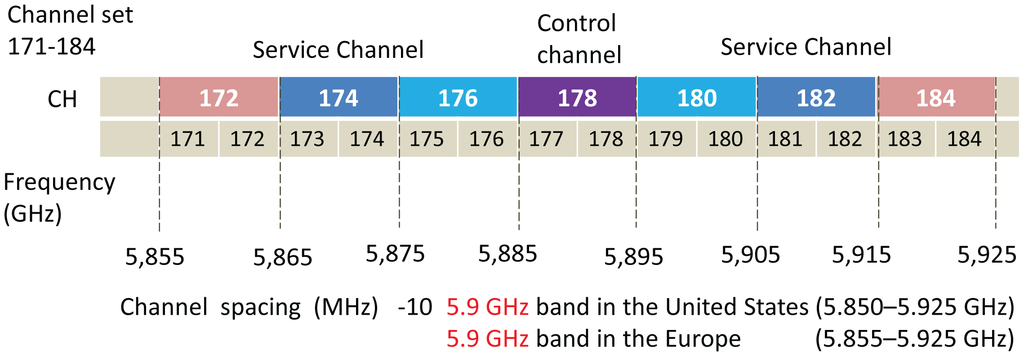
\includegraphics[width=0.70\textwidth]{fig/dsrc_spectrum.png}
    \caption{The DSRC Frequency Allocation in US}
    \label{fig:dsrc_spectrum}
\end{figure}
The seven channels are divided into 1 control channel (CCH) and 6 service channels (SCHs). The CCH is restricted to high-priority short message or data management and it is the only one shared between all WAVE devices. The first and the last channels of the spectrum are reserved for "public safety applications involving safety of life and property" \cite{fcc}.
\begin{figure} [H]
    \centering
    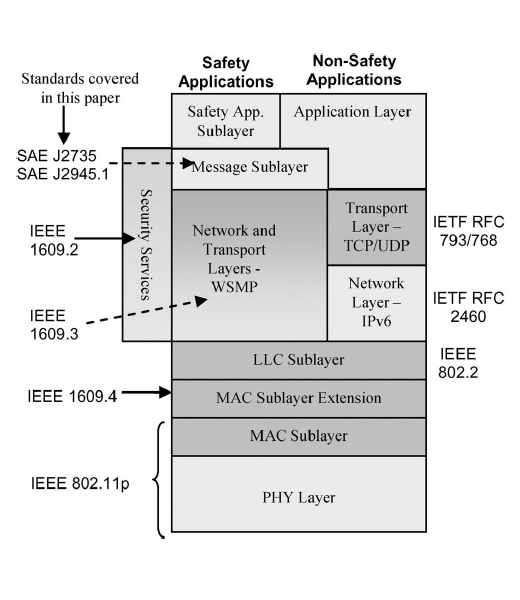
\includegraphics[width=0.50\textwidth]{fig/dsrc.png}
    \caption{DSRC architecture.}
    \label{fig:dsrc}
\end{figure}
\subsection{DSRC protocol stack}
As shown in \Cref{fig:dsrc} the DSRC architecture incorporates a number of protocols and corresponding standards. IEEE 802.11p provides the basic radio standard for DSRC. IEEE 802.11p is limited by the scope of IEEE 802.11, which is a MAC and PHY layer standard meant for single physical channel operation. The DSRC multi-channel setup and the operational concepts are taken care of by the upper layer IEEE 1609.x\cite{CJD_IEEE}.:
\begin{itemize}
	\item \emph{1609.1} Resource Manager: This standard provides a resource manager for WAVE, allowing communication between remote applications and vehicles.;
	\item \emph{1609.2} Security Services for Applications and Management Messages;
	\item \emph{1609.3} Networking Services: This standard addresses network layer issues in WAVE;
	\item \emph{1609.4} Multi-channel Operation: This standard deals with communications through multiple channels.
\end{itemize}
In particular, the IEEE 1609.3 \cite{1609.3} standard covers the WAVE connection setup and management. The IEEE 1609.4 \cite{1609.4} standard sits right on top of the IEEE 802.11p and enables operation of upper layers across multiple channels, without requiring knowledge of PHY parameters.\vskip 1em
The IEEE 802.11p physical layer is OFDM-based, and quite similar to the IEEE 802.11a physical layer design. The main difference is in the overall bandwidth used, which is \SI{10}{\MHz} for IEEE 802.11p instead of the 20 MHz of IEEE 802.11a. \vskip 1em
The IEEE 802.11p standard is meant to:
\begin{itemize}
    \item Describe the functions and services required by
WAVE-conformant stations to operate in a rapidly
varying environment and exchange messages without
having to join a Basic Service Set (BSS), as in the
traditional IEEE 802.11 use case.
    \item Define the WAVE signaling technique and interface
functions that are controlled by the IEEE 802.11
MAC.
\end{itemize}
\newpage

      \chapter{Simulation Frameworks}
\label{cha:frame}
Realistic simulations of IVC protocols are one of the main challenges in the VANET research domain. The ideal scenario is to perform an outdoor experiment, but setting up the vehicular network and running an outdoor experiment still has a high cost and potential safety issue. For example, in order to effectively evaluate the proposed system, we need many vehicles to communicate in a large road network, which may be costly and risky in real life.\\ In this field, network simulation environments, such as ns-3 and OMNeT++, are commonly used to model computer network configurations before they are deployed in the real world. Through simulation, the performance of different network setups can be compared, making it possible to recognize and resolve problems without conduct potentially expensive field tests.
As shown in \cite{mahajan2006urban} the quality of the results obtained by VANET simulations is heavily influenced by the quality of the mobility models.
\Cref{fig:mob} shown the evolution of mobility models \cite{sommer2008progressing}.
\begin{figure}[H]
    \centering
    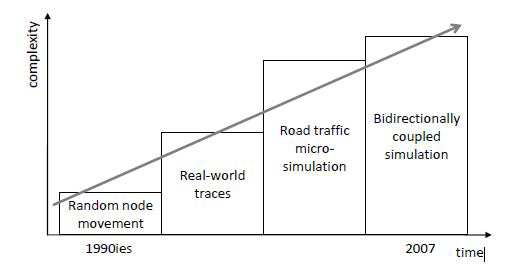
\includegraphics[width=0.7\textwidth]{fig/mobility.png}
    \caption{Evolution of mobility models}
    \label{fig:mob}
\end{figure}
Early approaches in mobility models relied on relatively simple models using random node movement \cite{johnson1996dynamic}.
Compared to the use of random mobility models, the modeling based on sets of pre-recorded real-world mobility trace was a crucial step towards realistic vehicle simulation. Such traces were obtained for example from the observation of city busses \cite{jetcheva2003design}. During network simulations, node mobility was controlled by synchronizing the position of the node in the simulation with the position of the vehicle stored in the trace file. \\
The difficulty on record trace data from real-world vehicle was overcame by generating movement traces artificially.
This way, artificial mobility models have the advantage of providing simulations with realistic mobility traces while at the same time allowing the freely adjustment of mobility parameters in order to understand their influence on simulations.\\
In case information about road congestion, accident, hazard warnings are transmitted over the network, a strictly interaction between the road traffic simulation and the network traffic is needed. \\
Bidirectionally coupled simulators like \cite{sommer2008need} provides not only more detailed insights into effects on network traffic, but at the same time have negligible impact on the run-time of simulations.
However, due to the on-the-fly node mobility computation,the results of the road traffic simulation cannot be re-used in form of trace files.
In bidirectional simulations, two inter-dependent processes are running concurrently, the network simulator and the road traffic simulator. The two processes share information like position and speed of the simulated nodes, while other data are local. The authors of \cite{sommer2008progressing} have analyzed the several mobility models and their impact.
In this thesis we decided to use Veins \cite{sommer2011bid} in combination with the network simulator OMNeT++ \cite{varga2001omnetpp} and the microscopic road traffic simulation package SUMO \cite{krajzewicz2002sumo}.
\section{Veins}
\label{sec:456}
Veins is an open source Inter-Vehicular Communication (IVC) simulation framework based on MiXiM \cite{kopke2008simulating} composed of an event-based network simulator and a road traffic micro simulation model. Both domains models are bi-directionally coupled and simulations are performed on-line. This way, not only the influence of road traffic on network traffic can be modelled, but also vice versa. In particular, the influences of IVC on road traffic can be modelled and complex interactions between both domains examined.\\
The framework is made up of two distinct simulators, OMNeT++ for network simulation and SUMO for road traffic simulation. \\
Veins includes a model of 802.11 that is tailored to use in vehicular networks, particularly IEEE 802.11p. This includes QoS channel access conforming to EDCA (that is, 4 queues with different access categories) and accurately captures frame timing, modulation and coding, and channel models.
Veins provides a comprehensive suite of IVC-specific models that can serve as a modular framework for simulating applications. Each model is contained in one or more of what OMNeT++ terms a \emph{module}, which can be instantiated in a running simulation to provide required functionality.
\section{Sumo}
\label{sec:Sumo}
Road traffic simulation models are classified into Macroscopic, Mesoscopic, and Microscopic models, according to the granularity with which traffic flows are examined. Macroscopic models model traffic at a large scale, while Mesoscopic model are concerned with the movement of whole platoons, using for example aggregated speed.density functions to model their behavior. However, simulations of VANETs scenarios are concerned with the accurate modelling of single radio transmission between a pair of nodes, so it require exact positions of simulated nodes. So, Mesoscopic and Macroscopic models cannot be used because they not offer this level of detail. \\
Traffic simulation in \emph{Veins} is performed by SUMO, which is a microscopic road traffic simulation package that uses the SK \cite{krauss1998microscopic} mobility model.
It can perform simulations both running with and without a GUI, and imports city maps from a variety of file formats.\\
SUMO allows high-performance simulations of huge networks with roads consisting of multiple lanes, as well as of intrajunction traffic on these roads, either using simple right-of-way rules or traffic lights. \\
Vehicle types are freely configurable with each vehicle following statically assigned routes, dynamically generated routes, or driving according to a configured timetable.
\section{OMNeT++}
OMNeT++ is a C++ based discrete event simulator for modeling communication networks, multiprocessors and other distributed or parallel systems. OMNeT++ is open-source, and it can be used either under the GNU General Public License or under its own license that also makes the software free for non-profit use.\\
Scenarios in OMNeT++ are represented by a hierarchy of reusable modules. Modules’ relationships and their communication links are stored as Network Description (NED) files and can be modeled graphically.\\ Typical ingredients of a NED description are simple module declarations, compound module definitions and network definitions. Simple module declarations describe the interface of the module: gates and parameters. Compound module definitions consist of the declaration of the module's external interface (gates and parameters), and the definition of sub-modules and their interconnection. A network definition basically defines a model as an instance of a module type. \\
Simulations are either run interactively, in a graphical environment, or are executed as command-line applications. The \emph{INET Framework} extension used in Veins, provides provides a set of OMNeT++ modules that represent various layers of the Internet protocol suite, e.g., the TCP, UDP, IPv4, and ARP protocols. It also provides modules that allow the modeling of spatial relations of mobile nodes and IEEE 802.11 transmissions between them.
\section{Connections}
\label{sec:Omnetpp}
\begin{figure}[H]
    \centering
    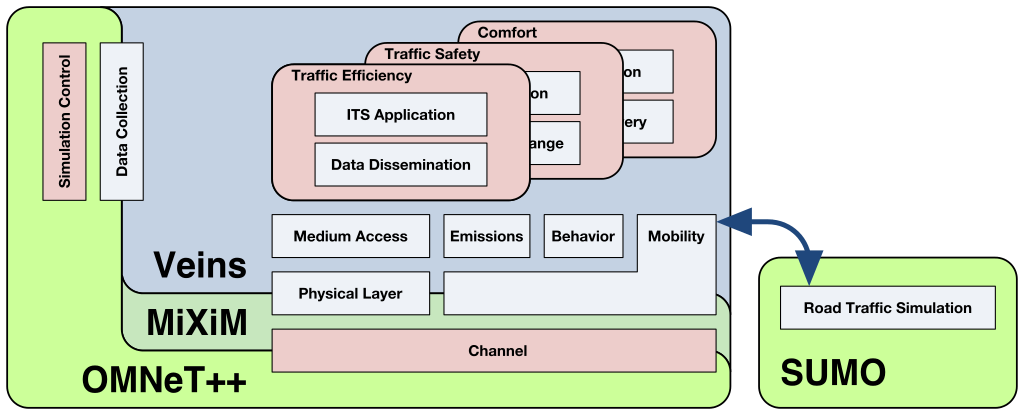
\includegraphics[width=0.7\textwidth]{fig/veins-arch.png}
    \caption{Structure of Veins}
\end{figure}
Each OMNeT++ node is associated with a network stack which includes an IEEE 802.11p wireless network interface provided by \emph{Veins}, plus a packet exchanging protocol and one or more applications.
To perform IVC evaluations, both simulators, OMNeT++ and SUMO, are running in parallel, connected via a TCP socket. \\The protocol for this communication has been standardized as the Traffic Control Interface (TraCI). This allows bi-directionally-coupled simulation of road traffic and network traffic. Movement of vehicles in the road traffic simulator SUMO is reflected in movement of nodes in an OMNeT++ simulation. Nodes can then interact with the running road traffic simulation, e.g. to simulate the influence of IVC on road traffic.\\
To do this, the control modules integrated with OMNeT++ and SUMO buffer any commands arriving within time steps in order to guarantee synchronous execution at each defined intervals. Every time step OMNeT++ then sends all commands to SUMO, at the end of the time step, SUMO would send a series of commands and the position of each vehicles to OMNeT++. Once it receive the commands it can reacts by introducing new nodes, by deleting the ones who had finished the simulation or by moving the nodes according to their road traffic simulation.\\
Using a simple request/response protocol, road traffic in SUMO can be influenced by OMNeT++ in different ways. Most importantly, time steps are generated to advance the simulation in SUMO. Furthermore, vehicles can be stopped to create artificial traffic jams, they can be resumed to
 resolve those jams, and each simulated vehicle can be individually rerouted around arbitrary road segments. This way, Veins accurately reflects how drivers that know about a traffic obstruction will try to avoid it. The sequence of messages exchanged between OMNeT++ and SUMO is shown in \Cref{fig:diagram}.
\begin{figure}[H]
    \centering
    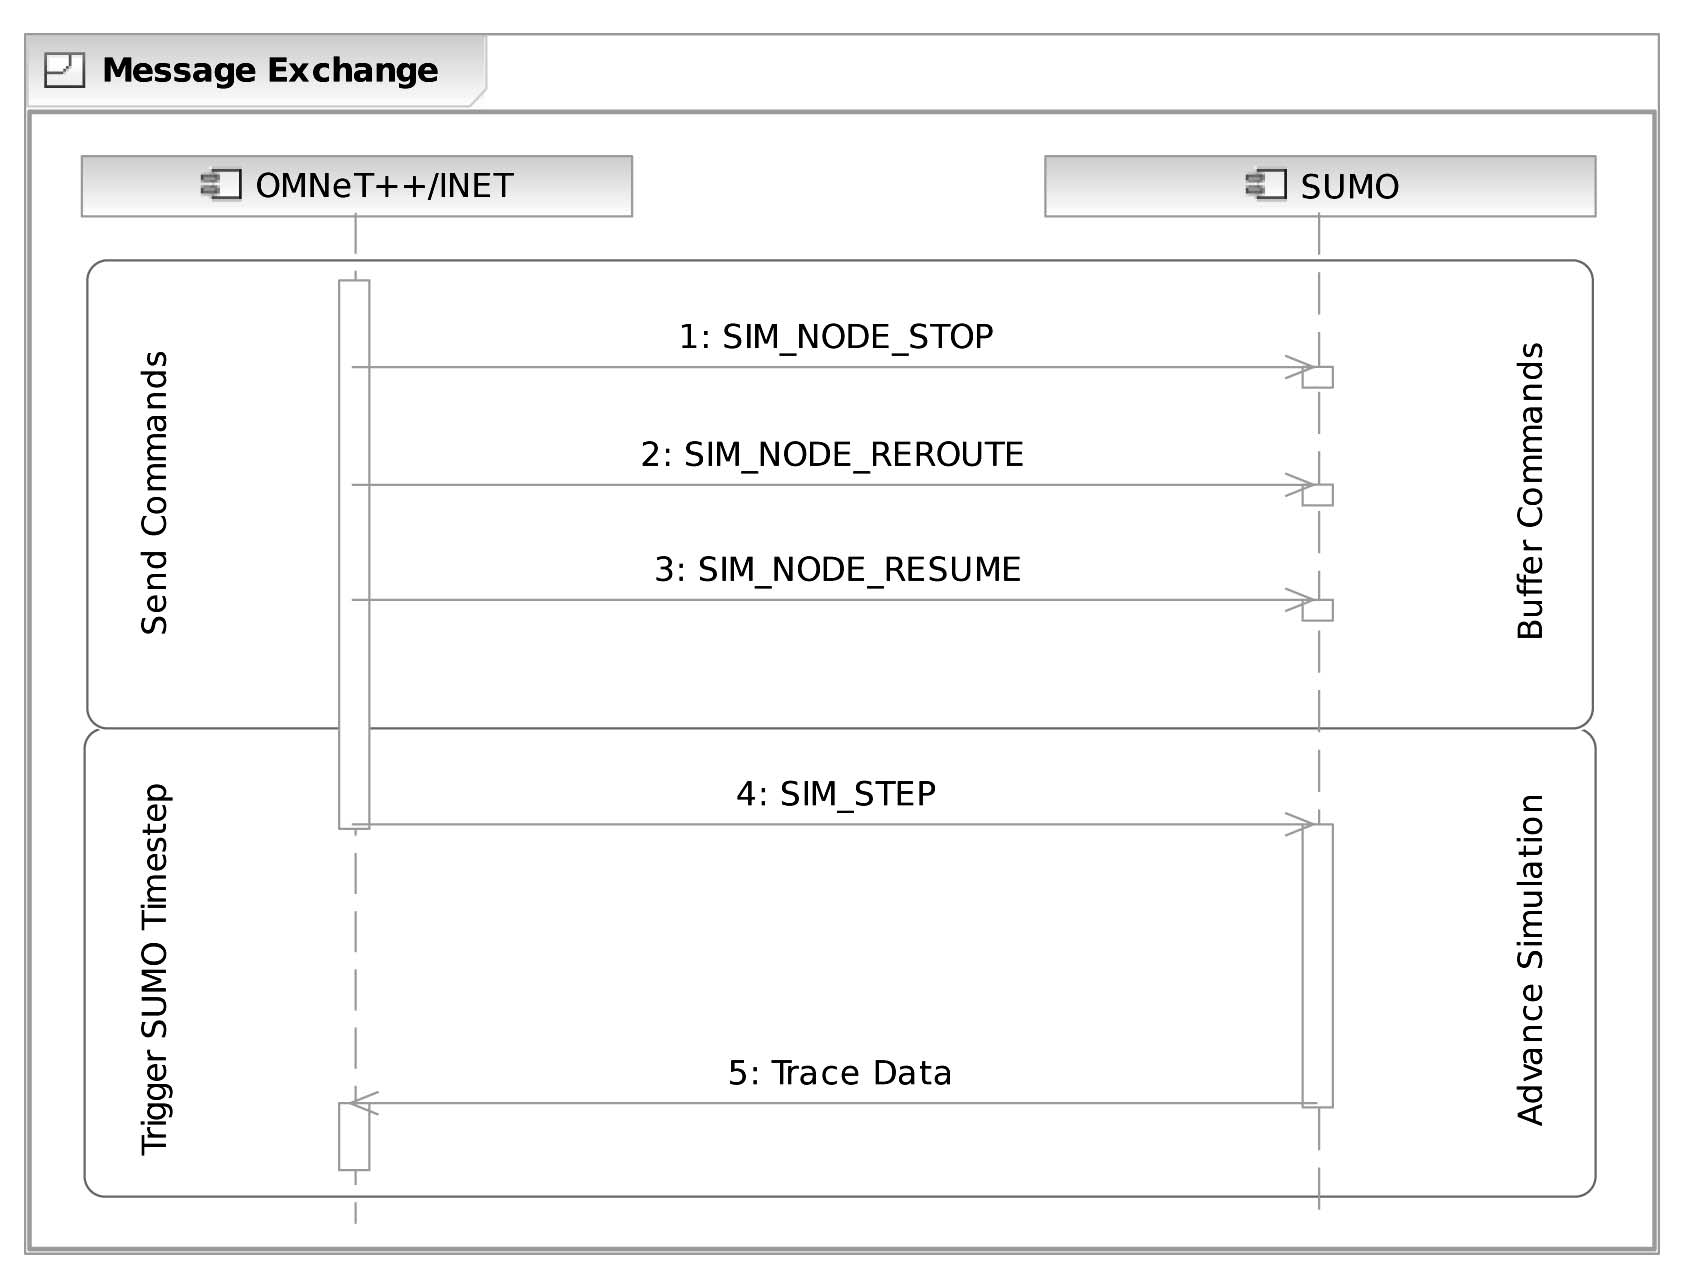
\includegraphics[width=0.7\textwidth]{fig/message-diagram.png}
    \caption{Sequence diagram of messages exchanged between network
    and road traffic simulator communication modules.}
    \label{fig:diagram}
\end{figure}
\newpage

      \chapter{Problem Statement}
\label{cha:PS}
\section{Mathematics Background}
\label{sec:MB}
The medium between the transmitting antenna of the sender and the receiving antenna of the receiver is generally called "channel". The characteristics of wireless signal changes as it travels from the sender to the receiver. These characteristics depend upon the distance between the two antennas, the paths taken by the signal, the existence of line of sight (LoS) paths between the two stations or the reflection, refraction and diffraction of the signal due to some objects in the paths. \\
In general, the power profile of the received signal can be obtained by convolving the power profile of the transmitted signal with the impulse response of the channel. Convolution in time domain is
equivalent to multiplication in the frequency domain. Therefore, the transmitted signal \textit{x}, after propagation through the channel \textit{H} becomes \textit{y}:
\begin{gather}
    y(f) = H(f)*x(f)+n(f)
\end{gather}

\textit{H(f)} is the channel response, and \textit{n(f)} is the noise. All the variable are all functions of the signal frequency \textit{f}.
The key components of the channel response are \textit{path loss}, \textit{shadowing} and \textit{multipath}.\vskip 1em
The simplest channel is the free space line of sight channel without objects between the receiver and
the transmitter or around the path between them. A convenient way to express the Free Space Path Loss is in terms of dB is:
\begin{gather}
    \text{FSPL}(\text{dB}) = 20\log\left(d\right) + 20\log\left(f\right)+ 20\log\left(\frac{4 \pi}{c}\right)
\label{eq:1}
\end{gather}
where:
\begin{itemize}
    \item $f$ is the signal frequency in \SI{}{\Hz};
    \item $d$ is the distance from the transmitter in \SI{}{\m};
    \item $c$ is the speed of light in \SI{}{\meter\per\second};
\end{itemize}\vskip 1em
If there are any objects along the path of the signal, some part of the transmitted signal is lost. This effect is called \textit{shadowing}. With shadowing the path loss becomes:
\begin{gather}
    \text{FSPL}(\text{dB}) = 20\log\left(d\right) + 20\log\left(f\right)+ 20\log\left(\frac{4 \pi}{c}\right) + \chi
\label{eq:2}
\end{gather}
Here $\chi$ is a normally distributed random variable which represent the effect of shadowing. As a result of shadowing, power received at the points that are at
the same distance d from the transmitter may be different and have a lognormal distribution. This
phenomenon is referred to as \textbf{lognormal shadowing}.\vskip 1em
The objects located in the environment of the wireless signal can reflect the signal. Some reflected waves are also received at the receiver. These reflected signals take different paths, so they arrive at the receiver with different amplitude and phase. These multiple signals can result in increased or decreased received power. \vskip 1em
Channel models can be characterized as deterministic or stochastic. Deterministic models are used for site-specific channel modeling; they consist of an environment model and a wave propagation model. The environment model describes position, geometry, material composition and surface properties of the wave propagation relevant objects and obstacles. The Maxwell equations, form the basis for all investigation of electromagnetic fields. In practical applications an analytic solution of the Maxwell equations it is not possible due to the high computation time. On the other hand, stochastic models can be computationally efficient and through probability distribution taken from statistical analyses of data collected from measurement campaigns, can emulate the main channel effects. \vskip 1em
In the field of stochastic communication channels Markov chains \cite{kemeny1960finite} are a powerful and commonly used tools. They consists of a finite number of states and corresponding state transition probabilities.\\
The Markov chain can be in one state at a time. The transition between states is governed by transition probability and takes place each time a digit is generated. If the state is not directly visible, but the output is visible the model is called \emph{hidden}.\vskip 1em
The availability of efficient algorithms for the extraction of HMM parameters from experimental data makes their application is vehicular communication simple and computationally inexpensive.\\
The use of Hidden Markov Chains in communication channels goes back to the model proposed by Gilbert \cite{gilbert1960capacity} in the 1960s.
\begin{figure} [H]
    \centering
    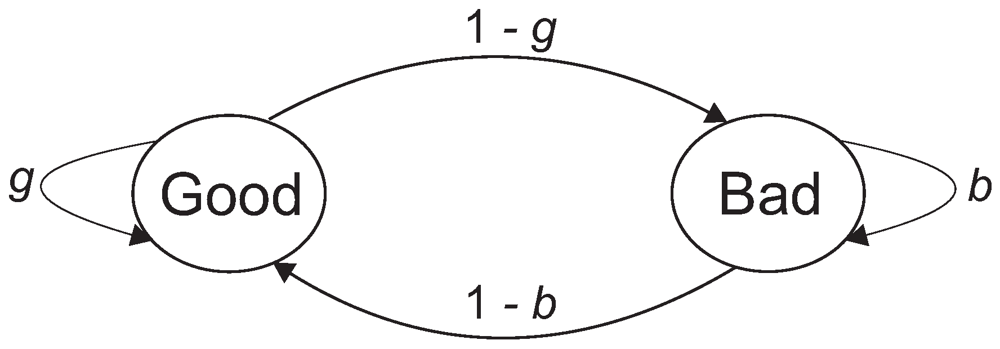
\includegraphics[width=0.5\textwidth]{fig/gilbert.png}
    \caption{The model proposed by Gilbert}
    \label{fig:gil}
\end{figure}
As can be seen in \Cref{fig:gil}, he proposed a chain with two state called \emph{Good} and \emph{Bad}. In the state Good the noise digit is always 0. In the state Bad a coin is tossed to decide whether the digit will be 0 or 1. To simulate burst noise, the states Bad and Good must tend to persist. So the probability of remaining in a state is larger than the probability of changing the state i.e. \textbf{\textit{g}} \textgreater\textgreater \textbf{\textit{1-g}} and \textbf{\textit{b}} \textgreater\textgreater \textbf{\textit{1-b}}. This can be avoided using a Continuous Time Markov Chain for which the time spent in each state is governed by non-negative real values with an exponential distribution.\vskip 1em
When modelling real-world vehicular channels a basic Gilbert's model with constant parameters should not be used, since the performance of the communication links is strongly dependent on the distance between nodes. To maintain an accurate representation of the propagation effects, the author of \cite{shivaldova2013vehicular} proposed to divide the measured error patterns into \emph{N} parts, corresponding to \emph{N} disjoint intervals of the same length. Once the parameters are estimated, they are combined to form a range-dependent Gilbert model, which has the same properties of the original, expect that the model parameters change according to the distance between the two vehicles.
\section{The Veins Framework Stack}
\subsection{Connection Manager}
The role of the \textbf{Connection Manager} module is to manage and coordinate the connections between all nodes. Nodes are connected with each other only when they are within the \textbf{maximal interference distance}. This distance is a bound on the maximal distance at which one nodes can still disturb the communication of a neighbor. To calculate the distance, the Connection Manager needs some parameters which are taken as input from the \textbf{omnetpp.ini} file, these are the max transmission power, the carrier frequency, the Path Loss coefficient and a sensitivity threshold, which is a lower bound on the received power, because a frame can never be decoded if its received power it is smaller than sensitivity threshold. \Cref{tab:param} below shows the parameters and the values used to compute the distance and used in each simulation.
\begin{table}[H]
    \centering
    {\tabulinesep=1.2mm
    \begin{tabu}{l|l}
        \hline
        Parameter & Value  \\
        \hline
        Max Transmission Power (pMax) & \SI{100}{\mW}$\sim$ \SI{20}{\dB}    \\
        Signal attenuation threshold (sat) & \SI{-94}{\dB} \\
        Path Loss coefficient ($\alpha$)  & 2.3 \\
        Carrier frequency (f)& \SI{5.890e+9}{\Hz} \\
        \hline
    \end{tabu}}
    \caption{Connection Manager parameters}
    \label{tab:param}
\end{table}
The module use the formula defined in \cite{sommer2012applicability}, which is derived from the \emph{Free Space path loss} model by introducing an additional environment-dependent path loss exponent $\alpha$, yielding
\begin{gather}
    A = 10\log\left(\left(\frac{4\pi f}{c}\right)^2 d^{\alpha}\right)
\label{eq:10}
\end{gather}
where \emph{d} is equal to the distance between the two antennas and \emph{c} is the speed of light measured in \si{\meter\per\second}. To compute the distance the equation has to be solved in the \emph{d} variable, yielding
\begin{gather}
    \newcommand*\rfrac[2]{{}^{#1}\!/_{#2}}
    d =\left(\frac{c^2 10^{\left(\frac{A}{10}\right)}}{16\pi^2 f^2}\right)^{\alpha^{-1}}
    \label{eq:4}
\end{gather}
using the parameters shown in \Cref{tab:param} and the attenuation $A$ equals to \SI{114}{\dB}, the resulting distance is \SI{751}{\meter}.
This means that in order to communicate, the distance between two vehicles has to be below \SI{751}{\meter}.\\
The Connection Manager will check every time the connections between a given vehicle and its neighbors, if the distance between the vehicle and a neighbor is below the interference distance the vehicles will remain neighbors, otherwise the Connection Manager will disconnect the two vehicles.\vskip 1em
The same thing is done when a new vehicle enter in the scenario, after the registration of the Nic, the Connection Manager will update the neighbors of the vehicle, while when the vehicle exit from the scenario, the Connection Manager will delete the Nic and disconnect the Nic with its old neighbors.
\subsection{Application and Protocol Layer}
In Veins each vehicle is provided with an \textbf{Application Layer} running on the top of the network stack and a \textbf{Protocol Layer} for the dissemination of the messages.
The role of the Application Layer is to load the parameters of the scenario, exchanging data with SUMO through the \textbf{TraCiCommandInterface} in order to dynamically set the parameters of each car or fetching the information of a car to synchronize it with the surrounding vehicles.\vskip 1em
Instead, the role of the Protocol Layer is to implement communication strategy to share information between the vehicles in the scenario, this includes choosing which kind of message has to be exchanged, insert in the messages information about position, speed, destination (manly broadcast) and so on and so forth. Both Application and Protocol Layers come with a basic class that provides primitives to allow an easier implementation of new protocols.
\subsection{Mac Layer}
The \textbf{Mac Layer} in Veins implements the specification described in the IEEE 1609.4 standards, which defines the multi-channel and Quality of Service (QoS) operation of radios, thus vehicles with a single radio will periodically switch between multiple channels.\vskip 1em
While there is only one Control Channel (CCH) to which every radio must tune for \SI{50}{\ms} in every \SI{100}{\ms}, there are others Service Channels (SCHs) on which a radio can transmit and receive in the remaining 50 ms time slots. Furthermore, to counter minor synchronization inexactness and to account for different frequency switching speeds of radios, a \SI{4} {\ms} guard interval at the beginning of every slot is added.\vskip 1em
When the Mac Layer receive a packet from the upper layer, it will assign the packet to one queue based on the channel type and the level of priority specified in the packet. Then a packet can be sent when the exponential back-off counter for its queue is 0 and the physical channel was idle for at least the time of one Arbitration Interframe Space (AIFS) which depends on the priority.\vskip 1em
When the packet is ready to be sent it will be encapsulated in a frame with the MAC address of both sender and receiver. To the frame will be attached also a \textbf{Signal} which stores the physical representation of the signal of an Physical Layer frame, this includes the start, duration and the propagation of the signal, and also the transmission power, bitrate, attenuations caused by effects of the channel on the signal during its transmission and the receiving power.\\
More information about the \textbf{Signal Module} can be found in \cite{kopke2008simulating}, while in \cite{eckhoff2012multichannel} the authors gives a deep prospective of the implementation of the Mac Layer.  \vskip 1em
On receiver side, when the Mac Layer receives a frame that is completely received and not noise from the Physical Layer, it will check the destination address and then send the frame to the upper layer. Also, the Physical Layer can send a control message to the Mac Layer to change the radio state if a transmission is over or changing the channel status to a specific value.
\subsection{Physical Layer}
The \textbf{Physical Layer} is directly connected to the Mac Layer via OMNeT++ channels and is able to send messages to other Physical Layers through sub-classing from \textbf{ChannelAcces}. Apart from message sending ans receiving, this layer acts as an interface between Physical Layer messages called \textbf{AirFrame} and the Analog Model and the Decider which are also initialized by this layer.\\
During the initialization, it will fetch the parameter from the \textbf{omnetpp.ini} and the \textbf{config.xml}, and then initialize the Analog Models and the Decider according to the parameters specified in the configuration files.\vskip 1em
When it receives a message from the upper layer, it will encapsulate the Mac Frame in a AirFrame and then send the frame down to the channel, which will send the frame to all the Nics connected with the sender.\vskip 1em
When receiving a message from the channel, the Physical Layer first passes the frame to the Analog Model and then it passes the message twice to the Decider, the first time at the beginning of the message and then at the end of the message. Once the decider has computed the bit error, the message has to be sent to the Mac Layer.\vskip 1em
Furthermore, the Physical Layer stores all the AirFrame in the \textbf{ChannelInfo} class which provides a function that returns all the AirFrame in the channel in a given intervals. This function is used by the Decider to calculate the Signal to Noise Ratio (SNR) and the Signal to Interference plus Noise Ratio (SINR) of a frame.
At the end, once a frame has been decoded and sent to the Mac Layer, it is deleted from the channel.
\subsection{Analog Model}
An \textbf{Analog Model} is a filter responsible for changing the attenuation value of a Signal. The attenuation of a Signal is calculated by implementations of fading, shadowing and path-loss models. An arbitrary number of analog models can be plugged into the Physical Layer. Each Analog Model is a filter class for Signals. The Analog Models which will be used and their parameters can be specified in the \textbf{config.xml}. Summing up the attenuation of all Analog Models gives the
attenuation part of the signal, which is calculated at the start of the reception of a message. Together with the sending power of a received packet the Decider can then compute the SNR and the SINR and, thus, bit errors.
\subsection{Decider}
The \textbf{Decider} has three main functions. The first time an AirFrame is parsed by the Decider, it will classify that AirFrame as a receivable messages or noise. The receiving power is calculated by multiplying the transmission power with the attenuation of every receiving Analog Model. If that power is under a sensitivity threshold specified in the \textbf{omnetpp.ini} then the frame will be treated as noise and it will not be decoded at its end. Also, a frame will not be decoded if the Nic is currently synced with another frame or the Radio State is in Transmission Mode.\vskip 1em
The latest time that the Decider can request the message from the Physical Layer is at the end of the receiving process of the message. This is also the time when the decider has to calculate the bit errors for the messages that are not treated as noise or interference. Depending on what are specified in the parameters, the Decider can compute both SINR and SNR or just the SINR. Compute both can be useful in order to understand if an error in the header or the payload of the frame is due to the interference of others frames in the channel in that interval or just to a collision, but on the other hand it will increase the computation time and so the simulation time. \vskip 1em
To compute the bit errors, the Decider requests all intersecting frames from the \textbf{ChannelInfo} and than compute the SINR or the SNR for that frame. The last task of the Decider is to provide information about the channel state. The Mac Layer can request the Decider to sense the channel for a certain amount of time. The decider then returns whether the channel is currently idle or busy.
\Cref{fig:scenario} shows an example of a possible scenario. Vehicles are disposed into a highway of four lanes. Vehicle A is sending a message to B with a distance of 20 meters. The neighbors of vehicle B are the vehicles within the circle. When vehicle B receives the frame from A, the Decider will compute the SINR or the SNR using the frames coming from its neighbors.
\begin{figure} [H]
    \centering
    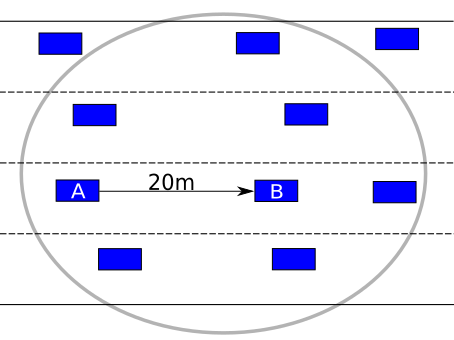
\includegraphics[width=0.6\textwidth]{fig/example.png}
    \caption{An example of scenario}
    \label{fig:scenario}
\end{figure}

\section{Problems and solutions}
\label{sec:prob}
While this approach gives the best results in term of accuracy, it can be really computationally expensive in term of simulation time. For example, thinking about a scenario with 640 vehicles, if each vehicle has more than 90 neighbors and the message propagation is governed by broadcast \textbf{beacons} sent by each vehicle to its neighbors every \SI{0.1}{\second}, in the channel there will be every second at least 500000 frames. This will obviously be extremely expensive due to the fact that to compute the SINR, the Decider will parse each frame in the channel at a given interval. \vskip 1em
To solve this problem, we proposed and implemented a Markov model with the aim to reduce the computation and maintain a good accuracy with respect to the original model. We developed a range and neighbors dependent Markov chain based on the Gilbert model explained in the first section of this chapter. The model is a CTMC, so the transition between the \textbf{Good} and \textbf{Bad} states is governed by two exponential variables whose values indicate the time spent in each state before the next transition.\vskip 1em
The choice of the granularity, i.e., the length of the interval in which the model parameters do not change, and the time spent in each states are essential for the accuracy of our range and neighbors modified Gilbert model. The granularity cannot be chosen arbitrarily small since dividing the measured error pattern into very short intervals will increase the computation of the parameters and there is the possibility that there are not enough data to estimate some intervals. On the other hand, estimating the model parameters for large intervals will inevitably reduce the computation but there is the possibility that the results do not reflect the distribution of the data used for the estimation.\vskip 1em
The data used for the estimation are a user behaviour. He can decide to use data that are taken by real experiment, extrapolating data from previous simulations or use randomly generated data to study the model under certain situations.
\section{Implementation}
\label{sec:implementation}
In order to implement the new model we modified some modules of the Veins Framework.\\
In the \textbf{ConnectionManager} we added the possibility to use a maximal interference distance specified by the user in the \textbf{omnetpp.ini} configuration file. Also we added the possibility to save the results of a simulation in a \textbf{CSV} file specified by the user in the configuration file. By default the file is structured as a tuple with information about the distance between the sender and the receiver, the number of neighbors of the receiver, if a packet has been correctly decoded or not, the IDs of the receiver and the sender and the simulation time of the recording.\vskip 1em
In the \textbf{Signal Module} we added two variable to store information about the distance between two vehicles and the list of neighbors of the receiver. Since this information will not be initialized in the Signal class, we added also four methods to store and fetch the information in a different module.\vskip 1em
In the \textbf{BasePhyLayer} in the \textbf{handleAirFrame} function, we fetched the neighbors of the receiver through the instance of the ConnectionManager and then we set the neighbors in the Signal via the function \textbf{setNeighbors} of the Signal class.\vskip 1em
In the \textbf{PhyLayer80211p} we added the initialization functions of the new Decider and the new Analog Model, also we added the possibility to schedule the recording intervals and a function that wrote the statistics received from the Decider in the csv. Since each vehicle has a own Physical Layer and they will write on the same csv, we decided to initialize the csv in the \textbf{ConnectionManager} which is global to each vehicle.\vskip 1em
The role of the new \textbf{Analog Model}, is to simply compute the distance between the receiver and the sender and then put it in the Signal through the method \textbf{setDistance}. The distance is not computed in the Physical Layer because it is needed only by the new model, so it is better to compute it in a new Module. If user needs the distance in the original model, he can simply add this new Analog Model the ones he is already using.\vskip 1em
The new \textbf{Decider} is the core of the new model. In the \textbf{config.xml} the user can insert the parameters of the Decider, these are: the center frequency of the channel, the intervals and the granularity of the model, the mean of the exponential variables representing the time spent in each state and the file that contains the parameters of the model. \\
Each Decider stores the channel's information between the receiver and the sender in an \textbf{HashMap} structured as follow: \textbf{$\left(\textit{sender\_id},\left(\textit{slotted distance,neighbors,channel state, next transition}\right)\right)$}.\\ When the Decider receives the frame from the Physical Layer for the first time, it will compute the slotted distance and then it will check if an entry with the Id of the sender is already in the map. If the map does not contain the entry, the Decider will add the sender to the map and set the next transition time as the actual simulation time plus the value of the transition from the Good state to the Bad state. \\
At the end of the receiving process of the message the Decider will compute the error rate of the frame. This will be only done if the frame is not under the minimum sensitivity.
If the distance and the neighbors between the two vehicles have been changed with respect to a previous communication between the two vehicles, the probability of being in a state or in another is based on the mean value of being in one of the two state. I.e. if the channel is on state Good at instant \textit{t}, the probability of being in the same state at instant \textit{t+1} is given by:
\begin{gather} \frac{\text{E[Good]}}{\text{E[Good]}+\text{E[Bad]}}
    \label{eq:5}
\end{gather}
while if the distance and the neighbors remain the same it means that the condition of the channel are not changed, and so the Decider will change the state of channel until the time of the next transition is larger than the actual simulation time, the following algorithm shows the computation of the actual state:\vskip 2em
\begin{center}
\begin{algorithm}[H]
    \caption{Compute State}
    $now\gets simTime\left(\right)$\;
    $P\textsubscript{Good}\gets \dfrac{E[Good]}{E[Good]+E[Bad]}$\;
    \eIf{$distance == old\_distance$ {\bf and} $neighbors == old\_neighbors$}
    {\While{$time\_to\_switch < now$}
        {\eIf{$state == Good$}
            {
            $time\_to\_switch \gets time\_to\_switch + \exp\left(\lambda\textsubscript{G}\right)$\;
                $state \gets Bad$\;
            }
            {
            $time\_to\_switch \gets           time\_to\_switch + \exp\left(\lambda\textsubscript{B}\right)$\;
                $state \gets Good$\;

            }
        }
    }
    {\eIf{$uniform\left(0,1\right) < P\textsubscript{Good}$}
        {
           $time\_to\_switch \gets SimTime\left(\right)$\;
            $state \gets Good$\;
        }
        {
            $time\_to\_switch \gets SimTime\left(\right)$\;
            $state \gets Bad$\;
        }
    }
\end{algorithm}
\end{center}\vskip 2em
At the end, the probability of correctly decode a frame is computed and the result is sent to the Physical Layer, which will write the result in the csv and send the frame to the upper layer.
\newpage

      \chapter{Evaluation}
\label{cha:eva}
The analysis of the new model was performed using \textbf{Plexe} \cite{segata2014plexe}. Plexe is an extension of Veins which permits the realistic simulation of platooning (i.e., automated car-following) systems. It features realistic vehicle dynamics and several cruise control models, permitting the analysis of control systems, large-scale and mixed scenario, as well as networking protocols and cooperative maneuvers. \vskip 1em
By default, Veins comes with a scenario that simulate the traffic in the city of Erlangen, Germany, while Plexe comes with a scenario that simulate an highway where the user can choose the number of lanes, the number of nodes in the network and the platoon size. This can extremely useful since different kind of simulations can be made. Furthermore, vehicles can be dynamically inserted or deleted from the network. In the scenario used for the tuning and the evaluation of the model, the cars are inserted using a fixed speed and a random distance from the preceding vehicle. The random distance is governed by a variable with a uniform distribution between \SI{10}{\m} and \SI{50}{\m}. When a vehicle is inserted, the distance from the preceding vehicle is computed by decreasing the position of the preceding vehicle in that lane by the result of the random variable and the length of the car, after that the Cruise Control speed is set to the one specified in the initialization and the CACC constant spacing is set to the distance between the car and the preceding car in its lane. Setting the CACC constant spacing is crucial, once the vehicle joins the network, the joiner notifies the leader that it is able to join the platoon. The leader sends back a confirmation and the joiner switches to CACC, closing its gap to the predecessor to the platoon inter-car distance.
Since the inter-car distance can be different from the computed distance between the two vehicles, the joiner can have a different distance, forcing the constant spacing can avoid this issue and so the distance will remain the same unless the Cruise Control speed is changed.\vskip 1em
The exchange of messages starts as soon as the vehicles join the network and it is governed by beacons sent by each vehicle to its neighbors every \SI{0.1}{\s}.
When sending the message, the Platooning Protocol fetch the speed, acceleration and the simulation time of the sender through the TraCICommandInterface and put them into the beacon, then the beacon is encapsulated into a Unicast Message and finally sent to the lower layer.\\
When the Platooning Application of the receiver receives the message, it will check if the beacon comes from a vehicle of the same platoon, if so it will update the its information according if the beacon comes from the leader of its platoon or from a preceding vehicle of its platoon. \vskip 1em
\section{Parameters Estimation}
\label{sec:estimation}
The estimation of the parameters has been made by running three simulations with 160, 320 and 640 vehicles in the scenario, and each simulation has been repeated 10 times with different a seed for the generation of the random numbers. The parameters used in the simulations are shown in \Cref{tab:param_simulations}.
\begin{table}[H]
    \centering
    {\tabulinesep=1.2mm
    \begin{tabu}{l|l}
        \hline
        Parameter & Value  \\
        \hline
        nCars & 160,320,640    \\
        platoonSize & 4 \\
        nLanes  & 4 \\
        platoonInsertSpeed& \SI{130}{\km\per\hour} \\
        startCommunication & Time Instant \\
        startCommunicationTime & \SI{0}{\s}\\
        communicationDuration & \SI{70}{\s}\\
        statStart & \SI{50}{\s}\\
        statInterval & \SI{10}{\s}\\
        leaderSpeed & \SI{130}{\km\per\hour} \\
        \hline
    \end{tabu}}
    \caption{The parameters used during the simulations}
    \label{tab:param_simulations}
\end{table}

The recording of the simulation is set to \SI{10}{\s} since recording all the simulation would be very expensive in term of memory used to store all the information.
\Cref{fig:original} shows the Analogue Model and the Decider used during the simulations with the original model.\vskip 3em
\begin{figure}[H]
\begin{lstlisting}[frame=bt, language=XML, numbers=none]
<root>
    <AnalogueModels>
        <AnalogueModel type="SimplePathlossModel">
            <parameter name="carrierFrequency" type="double" value="5.890e+9"/>
            <parameter name="alpha" type="double" value="2.3"/>
        </AnalogueModel>
        <AnalogueModel type="GenericFading">
            <parameter name="distribution" type="string" value="gaussian"/>
            <parameter name="param1" type="double" value="2.3"/>
        </AnalogueModel>
    </AnalogueModels>
    <Decider type="Decider80211p">
        <parameter name="centerFrequency" type="double" value="5.890e9"/>
    </Decider>
</root>
\end{lstlisting}
\caption{The XML configuration of the original model.}
\label{fig:original}
\end{figure}\vskip 2em
\Cref{fig:originalmodel} shows the results of the original model with 640 vehicles. The zones where there are not data are plotted in black. The plot is done using \textbf{Python}, grouping the results by the slotted distance and the number of neighbors. The distance is divided into 40 intervals with a range of \SI{20}{\m}. As can be seen the Packet Delivery Rate decrease with the increasing of the neighbors and the distance.\vskip 1em
Only the scenario with 640 vehicles is used to compute the distance, since merging all the 30 repetitions, i.e. 10 for each scenario, would be impossible due to an high RAM usage. As can be seen in the first plot, the probability of correctly receives a frame decreases with the increase of the distance and the neighbors.\vskip 1em
The extrapolation of the parameters has been made using \textbf{R}. First of all, the data are grouped by the distance and the neighbors. Then each interval is used to fit a weighted quadratic function, where weights are given by the occurrence of each possible neighbors in the interval. In fact, there can be neighbors that have an higher number of occurrences in respect to others neighbors, so it is correct to give different weights to different occurrences. Finally, the coefficients of each interval are printed in a csv file, which is then used by the new model.\vskip 1em With this approach the new model do not need to have different probabilities for the two state, since the probability of do not correctly decode a frame due to the Nic in Tx Mode or synced with another frame is already fitted in the function. The resulting function is the following:
\begin{gather}
    y=ax^2 + bx + c
\end{gather}
where:
\begin{itemize}
    \item $a$, $b$, $c$ are the coefficients of the intervals
    \item $x$ is the neighbors;
    \item $y$ is the probability of correctly receives a frame.
\end{itemize}
\begin{figure}[H]
    \centering
    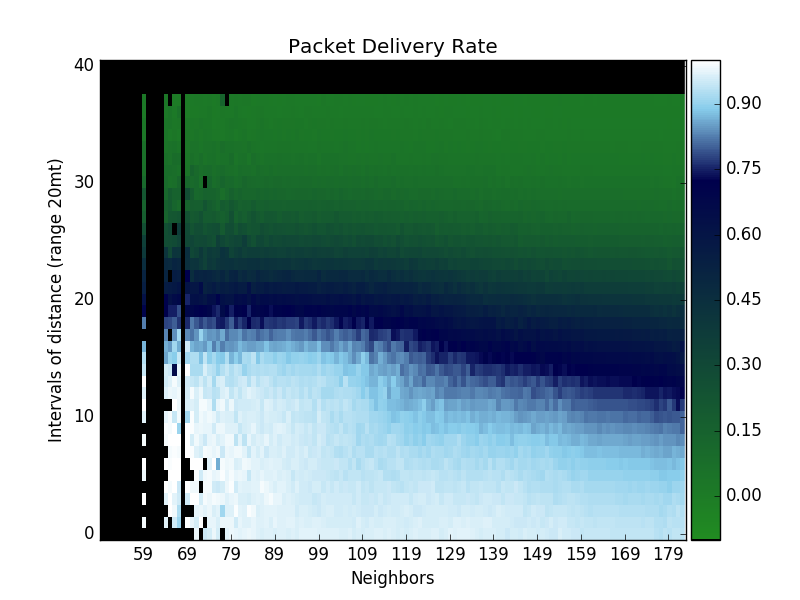
\includegraphics[width=0.8\textwidth]{fig/Original_640_plot.png}
    \caption{Packet Delivery Rate for each interval of distance and number of neighbors of the original model}
    \label{fig:originalmodel}
\end{figure}
\newpage
Once the parameters are estimated, the analysis of the two models was performed by running three simulation with 640 nodes per model. The Analogue Model and the Decider used for the new model are shown in \Cref{newmodel}.
\begin{figure}[H]
\begin{lstlisting}[frame=bt, language=XML, numbers=none]
<root>
    <AnalogueModels>
        <AnalogueModel type="ThesisAnalogueModel"></AnalogueModel>
    </AnalogueModels>
    <Decider type="ThesisDecider">
        <parameter name="centerFrequency" type="double" value="5.890e9"/>
        <parameter name="intervals" type="double" value="40"/>
        <parameter name="range" type="double" value="20"/>
        <parameter name="coefficients" type="string" value="coefficients.csv"/>
    </Decider>
</root>
\end{lstlisting}
\caption{The XML configuration of the new model.}
\label{newmodel}
\end{figure}
In order to have comparable results, the two simulations have to be dynamically equivalent. This means that at each instant the vehicles in the two simulations have to be in the same position, otherwise the two models cannot be compared. This is done by using the same seed for generating the random numbers. \vskip 1em
\section{Simulation efficiency gain}
\label{sec:gain}
The first metric analyzed is the efficiency gain of the new model with regards to the original model.
The analysis was performed by measuring the computational time while the communication between nodes is active. As described in \Cref{sec:prob}, the main problem of the original model is the computational time used during the computation of the SNR and the SINR. \vskip 1em
\subsection{Results}
\begin{table}[H]
    \centering
    {\tabulinesep=1.2mm
    \begin{tabu}{l|l l l|l}
        \hline
        Repetition & 1 & 2 & 3 & Mean \\
        \hline
           Original model &  \SI{16}{\hour} \SI{10}{\minute}  &  \SI{16}{\hour} \SI{20}{\minute}  &  \SI{16}{\hour} \SI{18}{\minute}  &  \SI{16}{\hour} \SI{16}{\minute}  \\
         New model & \SI{3}{\hour} \SI{50}{\minute} &  \SI{3}{\hour} \SI{55}{\minute}  &  \SI{3}{\hour} \SI{47}{\minute}  &  \SI{3}{\hour} \SI{51}{\minute}   \\
    \hline
        Decrease & $76\%$ & $76\%$ & $77\%$ & $76\%$ \\
        \hline
    \end{tabu}}
    \caption{Duration of the simulations}
    \label{tab:duration}
\end{table}
As can be seen from \Cref{tab:duration}, the mean duration of the new model is \SI{3}{\hour} \SI{51}{\minute}, while the original model takes on average \SI{16}{\hour} \SI{16}{\minute}. This means that there is a decrease of the $76\%$ in the computation time from the original to the new model.\vskip 1em
This could be an excellent result considering that the model can takes much less time in simulating very large and long scenario. For example, thinking at a scenario with an high number of nodes, where the user wants to study the packet exchanging during a day, it will take up to a week of simulation time, while with this model and appropriate parameters, the simulation will take barely two days of simulation.\vskip 1em
On the other hand it would be useless if there is a low accuracy between the two models. This brings to the second analysis explained in the following section.
\section{Accuracy analysis}
\label{sec:accuracy}
The second metric analyzed is the accuracy between the two models.
The analysis was performed by measuring for each pair of nodes, the number of correctly received packets of the two models and then measuring the differences using the Sample mean and the Standard deviation.
\subsubsection{Sample Mean}
The sample mean $\mu$ is given by the number of packets correctly received by a pair of vehicles in the new original, minus the number of packets correctly received by the same pair in the new model, thus are the number of packet that the original model has differently decoded in respect to the new model, a negative value means that the original model has correctly decoded fewer packets than the new model, while a positive value means that the original model has correctly decoded a greater number of packets than the new model. Then the result is normalized with respect to the total number of packets exchanged by the pair of nodes. Finally, the normalized value is divided by the total number of pairs.\\
Given the set of data $\chi = \left(x_1,x_2,..,x_n\right)$ with $x_i=\frac{b_i - a_i}{tot_i}$ where $b_i$ is the number of correctly received packets by the i-th pair of the original model, $a_i$ is the number of correctly received packets by the i-th pair of the new model and $tot_i$ is the total number of packets exchanged by the i-th pair. The sample mean is defined as:
\begin{gather}
\mu = \sum\limits_{i=1}^Nx_i\frac{1}{N}
    \label{eq:mean}
\end{gather}

The sample mean can be computed also using the absolute value $|\mu|$, yielding
\begin{gather}
    x_i=\frac{|b_i - a_i|}{tot_i}
    \label{eq:7}
\end{gather}
thus, the percentage of packets that the original model has differently decoded in respect to the new model.
\subsubsection{Standard Deviation}
The standard deviation $\sigma$ is a measure that is used to quantify the amount of variation of a set of data. In this measurement, the standard deviation measure the variation of packets differently decoded by the original model from the sample mean computed before. A standard deviation close to 0 indicates that the data points tend to be very close to the mean. Using the sample mean computed in \eqref{eq:mean}, the standard deviation is defined as:
\begin{gather}
    \sigma^2=\frac{1}{N-1}\sum\limits_{i=1}^N \left(x_i - \mu\right)^2
\end{gather}
\newpage
\begin{figure}[H]
    \centering
    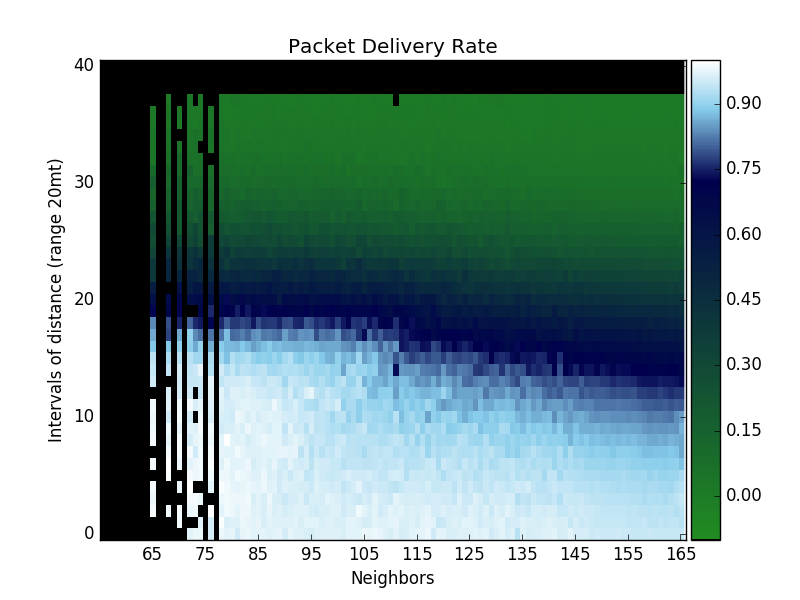
\includegraphics[width=0.8\textwidth]{fig/Original_test_640_plot.png}
    \caption{PDR of the original model in the evaluation.}
    \label{fig:pdro}
\end{figure}
\begin{figure}[H]
    \centering
    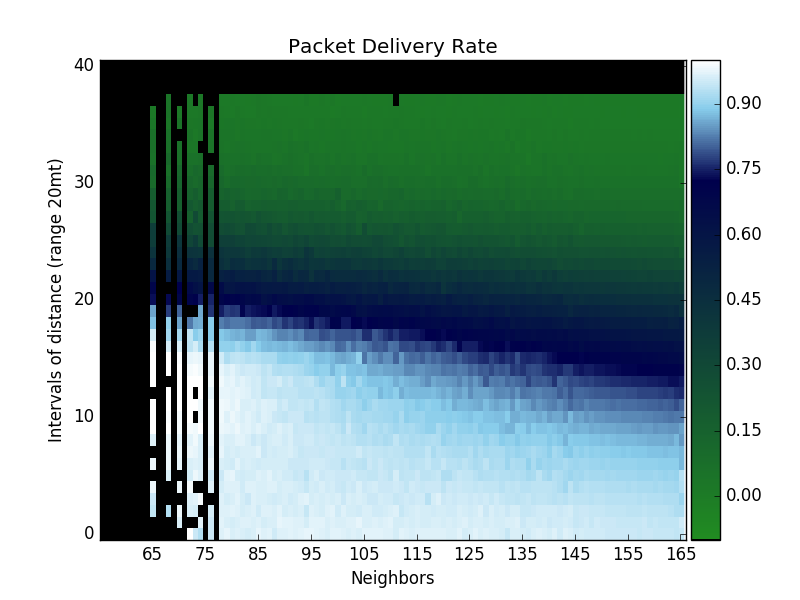
\includegraphics[width=0.8\textwidth]{fig/Markov_test_640_plot.png}
    \caption{PDR of the new model in the evaluation.}
    \label{fig:pdrn}
\end{figure}
\newpage
\subsection{Results}
\label{sec:Resultaccuracy}
\Cref{fig:pdro} and \Cref{fig:pdrn} show the PDR of the two model. As can be seen the two models have very similar results. The probability of correctly receives a packet decrease with the increasing of the neighbors and the distance.\\
As expected, a pair of vehicles that are very close have a very high probability of correctly receive a packet even if the receiver has an high number of neighbors.\\
\begin{table}[H]
    \centering
    {\tabulinesep=2.2mm
    \begin{tabu}{|l |l |l|}
        \hline
        $\mu$ & $|\mu|$ & $\sigma^2$  \\
        \hline
        $0.19\%$ & $2.53\%$ & $11.62\%$ \\
        \hline
    \end{tabu}}
    \caption{Result of accuracy measurement}
    \label{tab:accuracy}
\end{table}
As can be seen from \Cref{tab:accuracy} the results of the accuracy measurement, the two models have similar results. The result of the sample mean indicates that the original model correctly decoded in average $0.19\%$ packets more than the new model.\\
While the absolute value of the mean indicates that the original model decoded differently the $2.53\%$ of the packet with respect to the new model.\\
The standard deviation finally, indicates that there is a deviation of $11.62\%$ from the sample mean.
\newpage

      \chapter{Conclusions}
\vskip 1em
\label{cha:conclusion}
The new model presented in this thesis shows how it is possible to improve the performance of Veins with a range and neighbors dependent model.\vskip 1em
The first analysis reported in this thesis is the duration metric.
The analysis has shown that using the new model would substantially decrease the computation time, as the model do not have to compute the SNR and the SINR but only a probability given by the parameters of the model.\vskip 1em
The second analysis reported is the accuracy metric.
This analysis has shown that using the new model with parameters obtained from the original model lead to the same result of the original model.\vskip 1em
The two metric are obviously correlated, it would be useless to have a faster model but with results that does not reflect the reality. On the other hand it is useless to have a model that has the same accuracy of the original with only marginal gain in computation time.\\
As a possible application, the new model can be employed in long scenarios where the original model would spend days in computation.\\
As can be seen in this thesis, the two model can be used together. The original model can be used in short simulations to estimate the parameter of the new models and then the new model can be used in  longer simulations.\vskip 1em
A possible future enhancement can include some improvements in the computation of the PER, in fact if  the parameters do not cover the possibility to have frames not decoded due to Radio in wrong mode or frames not synced with the Nic, the new model would not even try to decode these frames and so it will process fewer frames.\\
It is possible to affirm that is could be a good starting point for those who will implement stochastic decisional model in Vehicular Networks using Veins.


    \endgroup


    % bibliografia in formato bibtex
    %
    % aggiunta del capitolo nell'indice
    % stile con ordinamento alfabetico in funzione degli autori
    \cleardoublepage
    \addcontentsline{toc}{chapter}{Bibliography}
    \bibliographystyle{ieeetr}
    \bibliography{biblio}
%%%%%%%%%%%%%%%%%%%%%%%%%%%%%%%%%%%%%%%%%%%%%%%%%%%%%%%%%%%%%%%%%%%%%%%%%%
%%%%%%%%%%%%%%%%%%%%%%%%%%%%%%%%%%%%%%%%%%%%%%%%%%%%%%%%%%%%%%%%%%%%%%%%%%
%% Nota
%%%%%%%%%%%%%%%%%%%%%%%%%%%%%%%%%%%%%%%%%%%%%%%%%%%%%%%%%%%%%%%%%%%%%%%%%%
%% Nella bibliografia devono essere riportati tutte le fonti consultate
%% per lo svolgimento della tesi. La bibliografia deve essere redatta
%% in ordine alfabetico sul cognome del primo autore.
%%
%% La forma della citazione bibliografica va inserita secondo la fonte utilizzata:
%%
%% LIBRI
%% Cognome e iniziale del nome autore/autori, la data di edizione, titolo, casa editrice, eventuale numero dell’edizione.
%%
%% ARTICOLI DI RIVISTA
%% Cognome e iniziale del nome autore/autori, titolo articolo, titolo rivista, volume, numero, numero di pagine.
%%
%% ARTICOLI DI CONFERENZA
%% Cognome e iniziale del nome autore/autori (anno), titolo articolo, titolo conferenza, luogo della conferenza (città e paese), date della conferenza, numero di pagine.
%%
%% SITOGRAFIA
%% La sitografia contiene un elenco di indirizzi Web consultati e disposti in ordine alfabetico.
%% E’ necessario:
%%   Copiare la URL (l’indirizzo web) specifica della pagina consultata
%%   Se disponibile, indicare il cognome e nome dell’autore, il titolo ed eventuale sottotitolo del testo
%%   Se disponibile, inserire la data di ultima consultazione della risorsa (gg/mm/aaaa).
%%%%%%%%%%%%%%%%%%%%%%%%%%%%%%%%%%%%%%%%%%%%%%%%%%%%%%%%%%%%%%%%%%%%%%%%%%
%%%%%%%%%%%%%%%%%%%%%%%%%%%%%%%%%%%%%%%%%%%%%%%%%%%%%%%%%%%%%%%%%%%%%%%%%%


    \titleformat{\chapter}
        {\normalfont\Huge\bfseries}{Allegato \thechapter}{1em}{}
    % sezione Allegati - opzionale

\end{document}
